% \VignetteDepends{stats}
% \VignetteIndexEntry{qvalue Tutorial}
% \VignetteKeywords{Significance Analysis}
% \VignettePackage{qvalue}
\documentclass[11pt]{article}

\usepackage{epsfig}
\usepackage{latexsym}
\usepackage{amsmath}
\usepackage{amssymb}
\usepackage{amsfonts}
\usepackage{amsxtra}
\usepackage{graphicx,subfigure}
\usepackage{vmargin}

\newcommand{\Robject}[1]{{\texttt{#1}}}
\newcommand{\Rfunction}[1]{{\texttt{#1}}}
\newcommand{\Rpackage}[1]{{\texttt{#1}}}
\newcommand{\Rclass}[1]{{\texttt{#1}}}
\newcommand{\Rmethod}[1]{{\texttt{#1}}}
\newcommand{\Rfunarg}[1]{{\texttt{#1}}}

\parindent 0in
\setpapersize{USletter}
\setmarginsrb{1truein}{0.5truein}{1truein}{0.5truein}{16pt}{30pt}{0pt}{20truept}
\setlength{\emergencystretch}{2em}
\usepackage{/Library/Frameworks/R.framework/Resources/share/texmf/Sweave}
\begin{document}

\title{Bioconductor's qvalue package}
\author{Alan Dabney and John Storey \\
Department of Biostatistics \\
University of Washington \\
email: \texttt{jstorey@u.washington.edu}}

\maketitle
\bibliographystyle{plain}
\tableofcontents

% library(tools)
% Rnwfile <- file.path("c:/alan/biostat/storey/fdr/package/vignette", "qvalue.Rnw") 
% Sweave(Rnwfile)

\section{Overview}

The \Rpackage{qvalue} package contains functions for the computation and presentation of q-values for 
features from an experiment with multiple comparisons.  A q-value is a measure of significance for a 
particular feature, analagous to a p-value.  However, where the p-value assigns significance in terms 
of the false positive rate, the q-value assigns significance in terms of the false discovery rate.  See 
\cite{storey:tibs:2003} for more detailed information.\\

This document provides a tutorial for using the \texttt{qvalue} package.  The package consists of four 
functions (\Rfunction{qvalue} for computing q-values from p-values, \Rfunction{qplot} for visualizing the 
results with graphs, \Rfunction{qsummary} for visualizing the results with a table, and \Rfunction{qwrite} for 
writing the output to file) and a GUI (\Rfunction{qvalue.gui}).  As with any R package, detailed information 
on functions, their arguments and value, can be obtained in the help files. For instance, to view the help 
file for the function \Rfunction{qvalue} within R, type \texttt{? qvalue}. \\

\section{Case study: the breast cancer dataset of Hedenfalk et al. (2001)}

We demonstrate the functionality of this package using gene expression data from the breast cancer study 
of \cite{hedenfalk:etal:2001}.  Comparison was made between two types of genetic mutation that are 
associated with an increased risk of breast cancer, BRCA1 and BRCA2.  There were 7 and 8 cDNA arrays for 
BRCA1 and BRCA2, respectively.  The example considered here is restricted to $3,170$ genes as described 
in \cite{storey:tibs:2003}.  A 2-sample t-statistic was used to compare the two mutation types, gene by 
gene, and p-values were assigned by a permutation-based simulation of the null distribution.  The original 
data and code for preprocessing can be found at 

\begin{center}
\texttt{http://faculty.washington.edu/$\sim$jstorey/qvalue/results.html}.
\end{center}

The p-values from the BRCA1/BRCA2 analysis are included with the \Rpackage{qvalue} package as the dataset 
\texttt{hedenfalk}.  To obtain the p-values, type \texttt{data(hedenfalk)}, and to view a description of 
the experiments and data, type \texttt{? hedenfalk}.  We also check the length of the p-value vector and plot 
a histogram.\\  

\begin{Schunk}
\begin{Sinput}
> library(qvalue)
> data(hedenfalk)
> length(hedenfalk)
\end{Sinput}
\begin{Soutput}
[1] 3170
\end{Soutput}
\end{Schunk}

\begin{Schunk}
\begin{Sinput}
> hist(hedenfalk)
\end{Sinput}
\end{Schunk}

\section{The \Rfunction{qvalue} function}

The \Rfunction{qvalue} function computes q-values from the p-values of an experiment with multiple comparisons.  
We assign the output of the function call to the object \texttt{qobj} and plot a histogram of the q-values.

\begin{Schunk}
\begin{Sinput}
> qobj <- qvalue(hedenfalk)
\end{Sinput}
\end{Schunk}

\begin{Schunk}
\begin{Sinput}
> hist(qobj$qvalues)
\end{Sinput}
\end{Schunk}

\section{The \Rfunction{qsummary} function}

The \Rfunction{qsummary} function reports an estimate ($\pi_0$) of the proportion of genes for which the null 
hypothesis is true, and presents a table comparing p-values to q-values.

\begin{Schunk}
\begin{Sinput}
> qsummary(qobj)
\end{Sinput}
\begin{Soutput}
Call:
qvalue(p = hedenfalk)

pi0:	0.6681177	

Cumulative number of significant calls:

        <1e-04 <0.001 <0.01 <0.025 <0.05 <0.1   <1
p-value     15     76   265    424   605  868 3170
q-value      0      0     1     73   162  319 3170
\end{Soutput}
\end{Schunk}

\section{The \Rfunction{qplot} function}

The \Rfunction{qplot} function produces four plots:
\begin{itemize}
\item A plot of $\pi_0$ versus the tuning parameter $\lambda$ (see \cite{storey:tibs:2003}).
\item A plot comparing p-values to q-values.
\item A plot of the number of significant genes by q-value.
\item A plot of the number of expected false positives by the number of significant genes.
\end{itemize}

\begin{Schunk}
\begin{Sinput}
> qplot(qobj)
\end{Sinput}
\end{Schunk}

\section{The \Rfunction{qwrite} function}

The \Rfunction{qwrite} function writes the output of the function \texttt{qvalue} to a file.  If all defaults 
were chosen in the call to \Rfunction{qvalue}, the output file contains $\pi_0$ in the first row and 
a $3,071 \times 2$ matrix of p- and q-values in the rest.  Note that \Rfunction{qwrite} writes to the file 
``my-qvalue-results.txt'' in the working directory by default.  The file name and location can be specified 
with the \Rfunarg{filename} argument to \Rfunction{qwrite}.

\begin{Schunk}
\begin{Sinput}
> qwrite(qobj)
\end{Sinput}
\end{Schunk}

\section{The \Rfunction{qvalue.gui} GUI}

The \Rfunction{qvalue.gui} function launches a GUI with which you can conduct all the tasks described above.  
The GUI is described in full detail in the accompanying manual.  It is launched by typing 
\texttt{qvalue.gui()}.

\bibliography{qvalue} 

\begin{figure}[ht]
  \begin{center}
    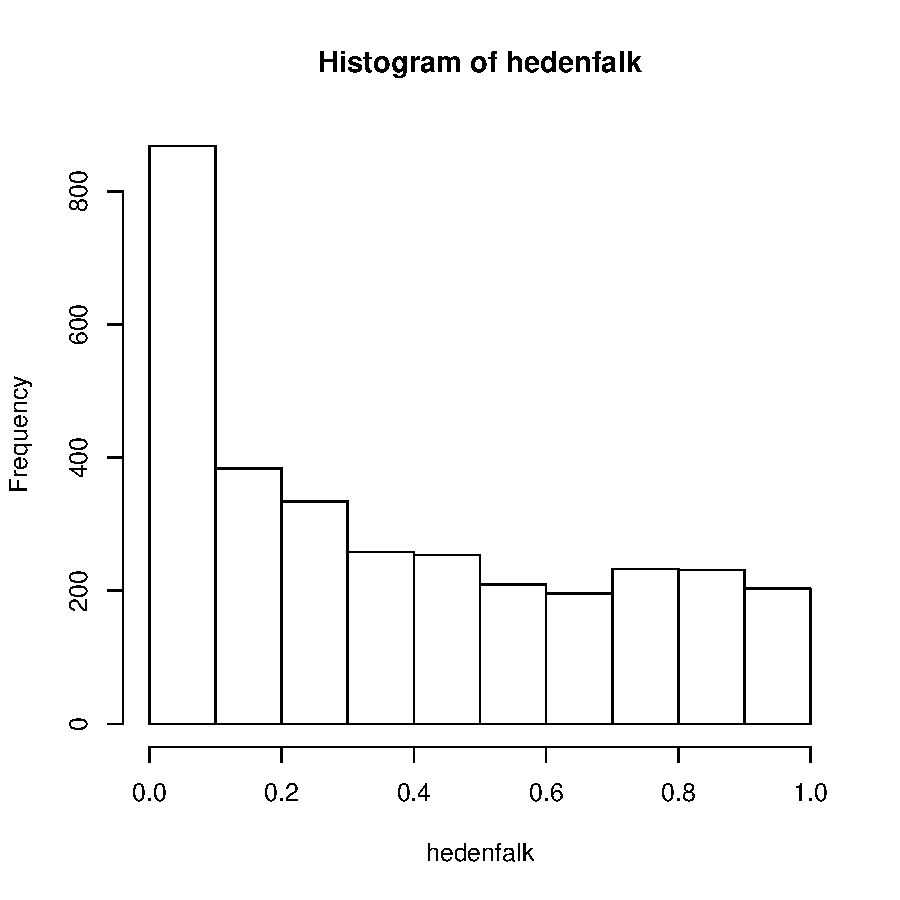
\includegraphics[width=5in,height=5in]{pHist}
  \end{center}
  \caption{Histogram of p-values.}
\end{figure}

\begin{figure}[ht]
  \begin{center}
    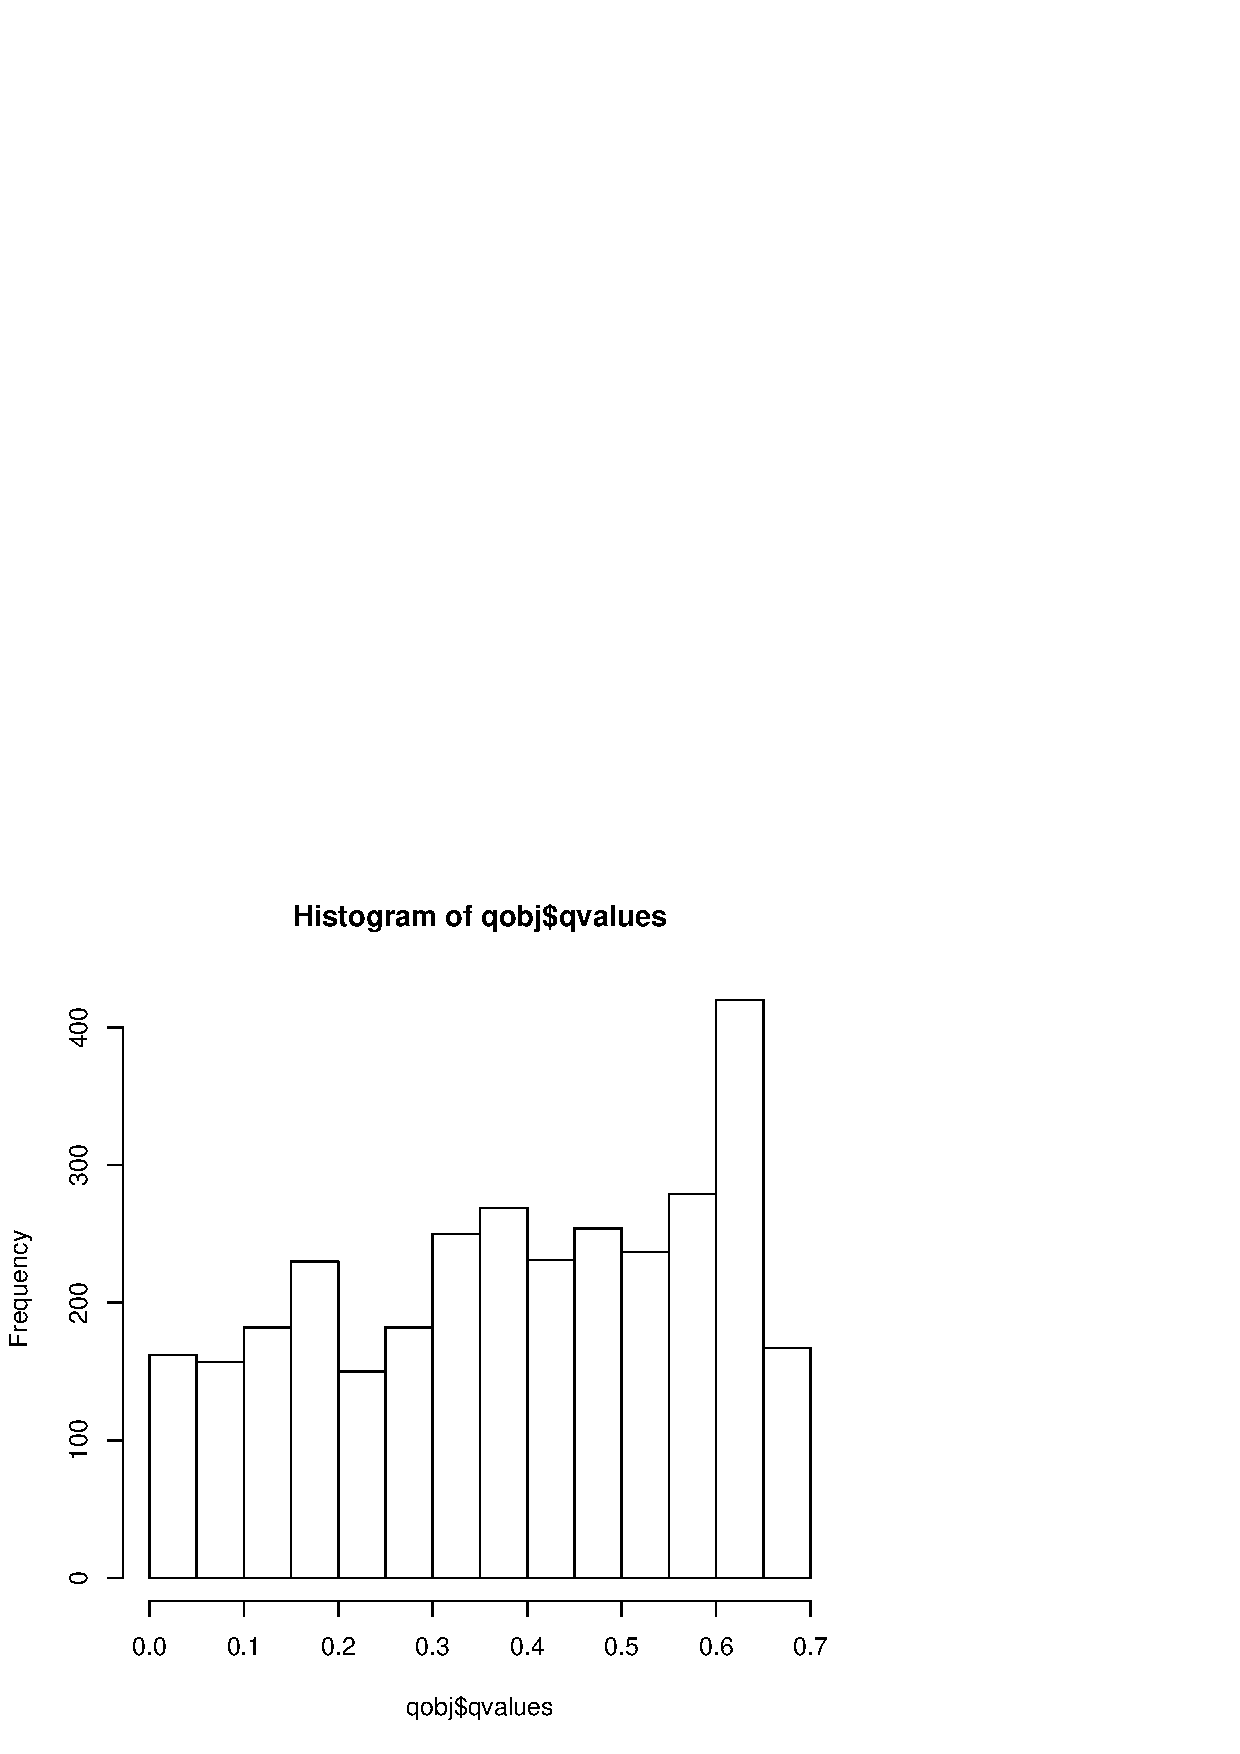
\includegraphics[width=5in,height=5in]{qHist}
  \end{center}
  \caption{Histogram of q-values.}
\end{figure}

\begin{figure}[ht]
  \begin{center}
    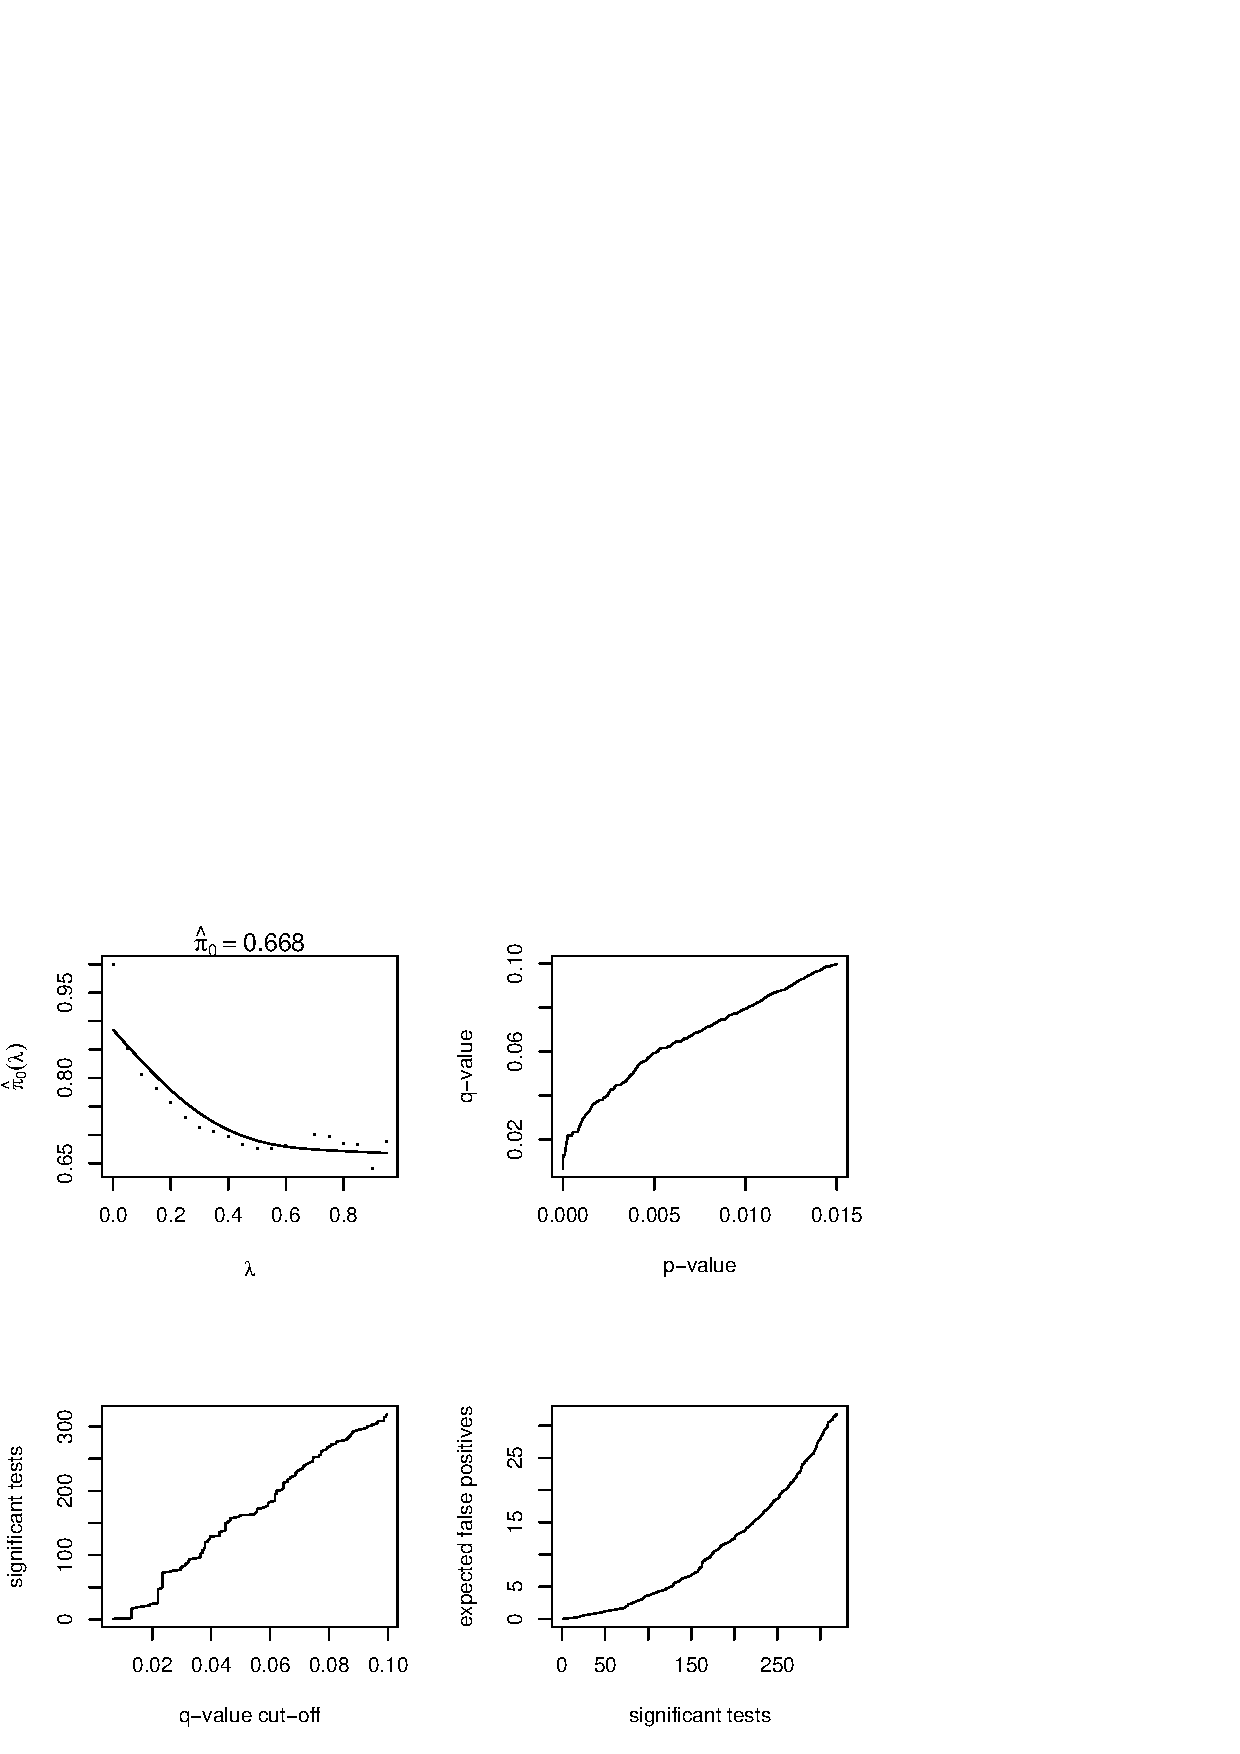
\includegraphics[width=5in,height=5in]{qPlots}
  \end{center}
  \caption{Miscellaneous plots.}
\end{figure}

\end{document}
